\documentclass[12pt,a4paper]{article}

\input{../preamble_files/packages}
\input{../preamble_files/figures}
\input{../preamble_files/references}
\input{../preamble_files/shortcuts}
\input{../preamble_files/listings}

\pagestyle{fancy}
\lhead{Richard Whitehill}
\chead{MATH 551 -- HW 1}
\rhead{02/10/22}
\cfoot{\thepage~of~\pageref{LastPage}}

\newcommand{\prob}[2]{\textbf{#1)} #2}

\setlength{\parskip}{\baselineskip}
\setlength{\parindent}{0pt}

\begin{document}

\prob{1}{Prove that the following equations have at least one solution in the given intervals.}

(a) $x - (\ln{x})^3 = 0,\quad [5,7]$

(b) $5x\cos(\pi x) - 2x^2 + 3 = 0,\quad [0,2]$

\prob{2}{Verify that the function $|| \cdot ||_1$ defined on $\reals^n$ by
\begin{align*}
||x|| = \sum_{i=1}^{n} |x_i|
\end{align*}
is a norm on $\reals^n$.}

\prob{3}{Find $l_1,~l_2,~\text{ and }l_{\infty}$ norms of the following vectors or matrices.}

(a) $x = (2,1,-3,4)^{T}$

(b) $x = (\sin{k},\cos{k},2^{k})^{T}$

(c) 
\[
\begin{bmatrix}
10 & 15 \\
0  & 1
\end{bmatrix}
\]

(d) 
\[
\begin{bmatrix}
2 & -1 & 0 \\
-1 & 2 & -1 \\
0 & -1 & 2
\end{bmatrix}
\]

\prob{4}{Taylor expand the following function.}

(a) $e^x$ around $x = 0$
\begin{align*}
e^{x} = 1 + x + \frac{x^{2}}{2} + \frac{x^{3}}{6} + \frac{x^{4}}{24} + \frac{x^{5}}{120} + \frac{x^{6}}{720} + \frac{x^{7}}{5040} + O\left(x^{8}\right)
\end{align*}

(b) $\log(x+1)$ around $x = 0$
\begin{align*}
\log(x+1) = x - \frac{x^{2}}{2} + \frac{x^{3}}{3} - \frac{x^{4}}{4} + \frac{x^{5}}{5} - \frac{x^{6}}{6} + \frac{x^{7}}{7} + O\left(x^{8}\right)
\end{align*}

\inputpython{prob4.py}

\prob{5}{Plot the function $e^x$ on $[0,1]$ in a black solid line. On the same graph, plot the function $1+x+\frac{x^2}{2!}$ in blue circle.}

\bef
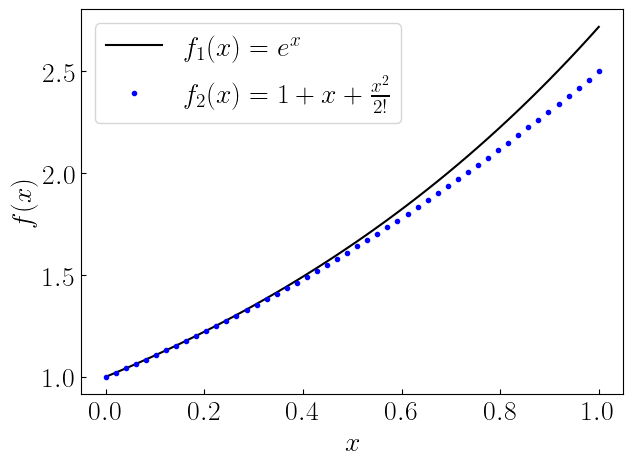
\includegraphics[scale=0.75]{prob5fig.png}
\eef

\inputpython{prob5.py}



\end{document}
